\section{A kapcsolás}

\subsection{Rendszerdiagram}
\begin{figure}[H]
	\centering
	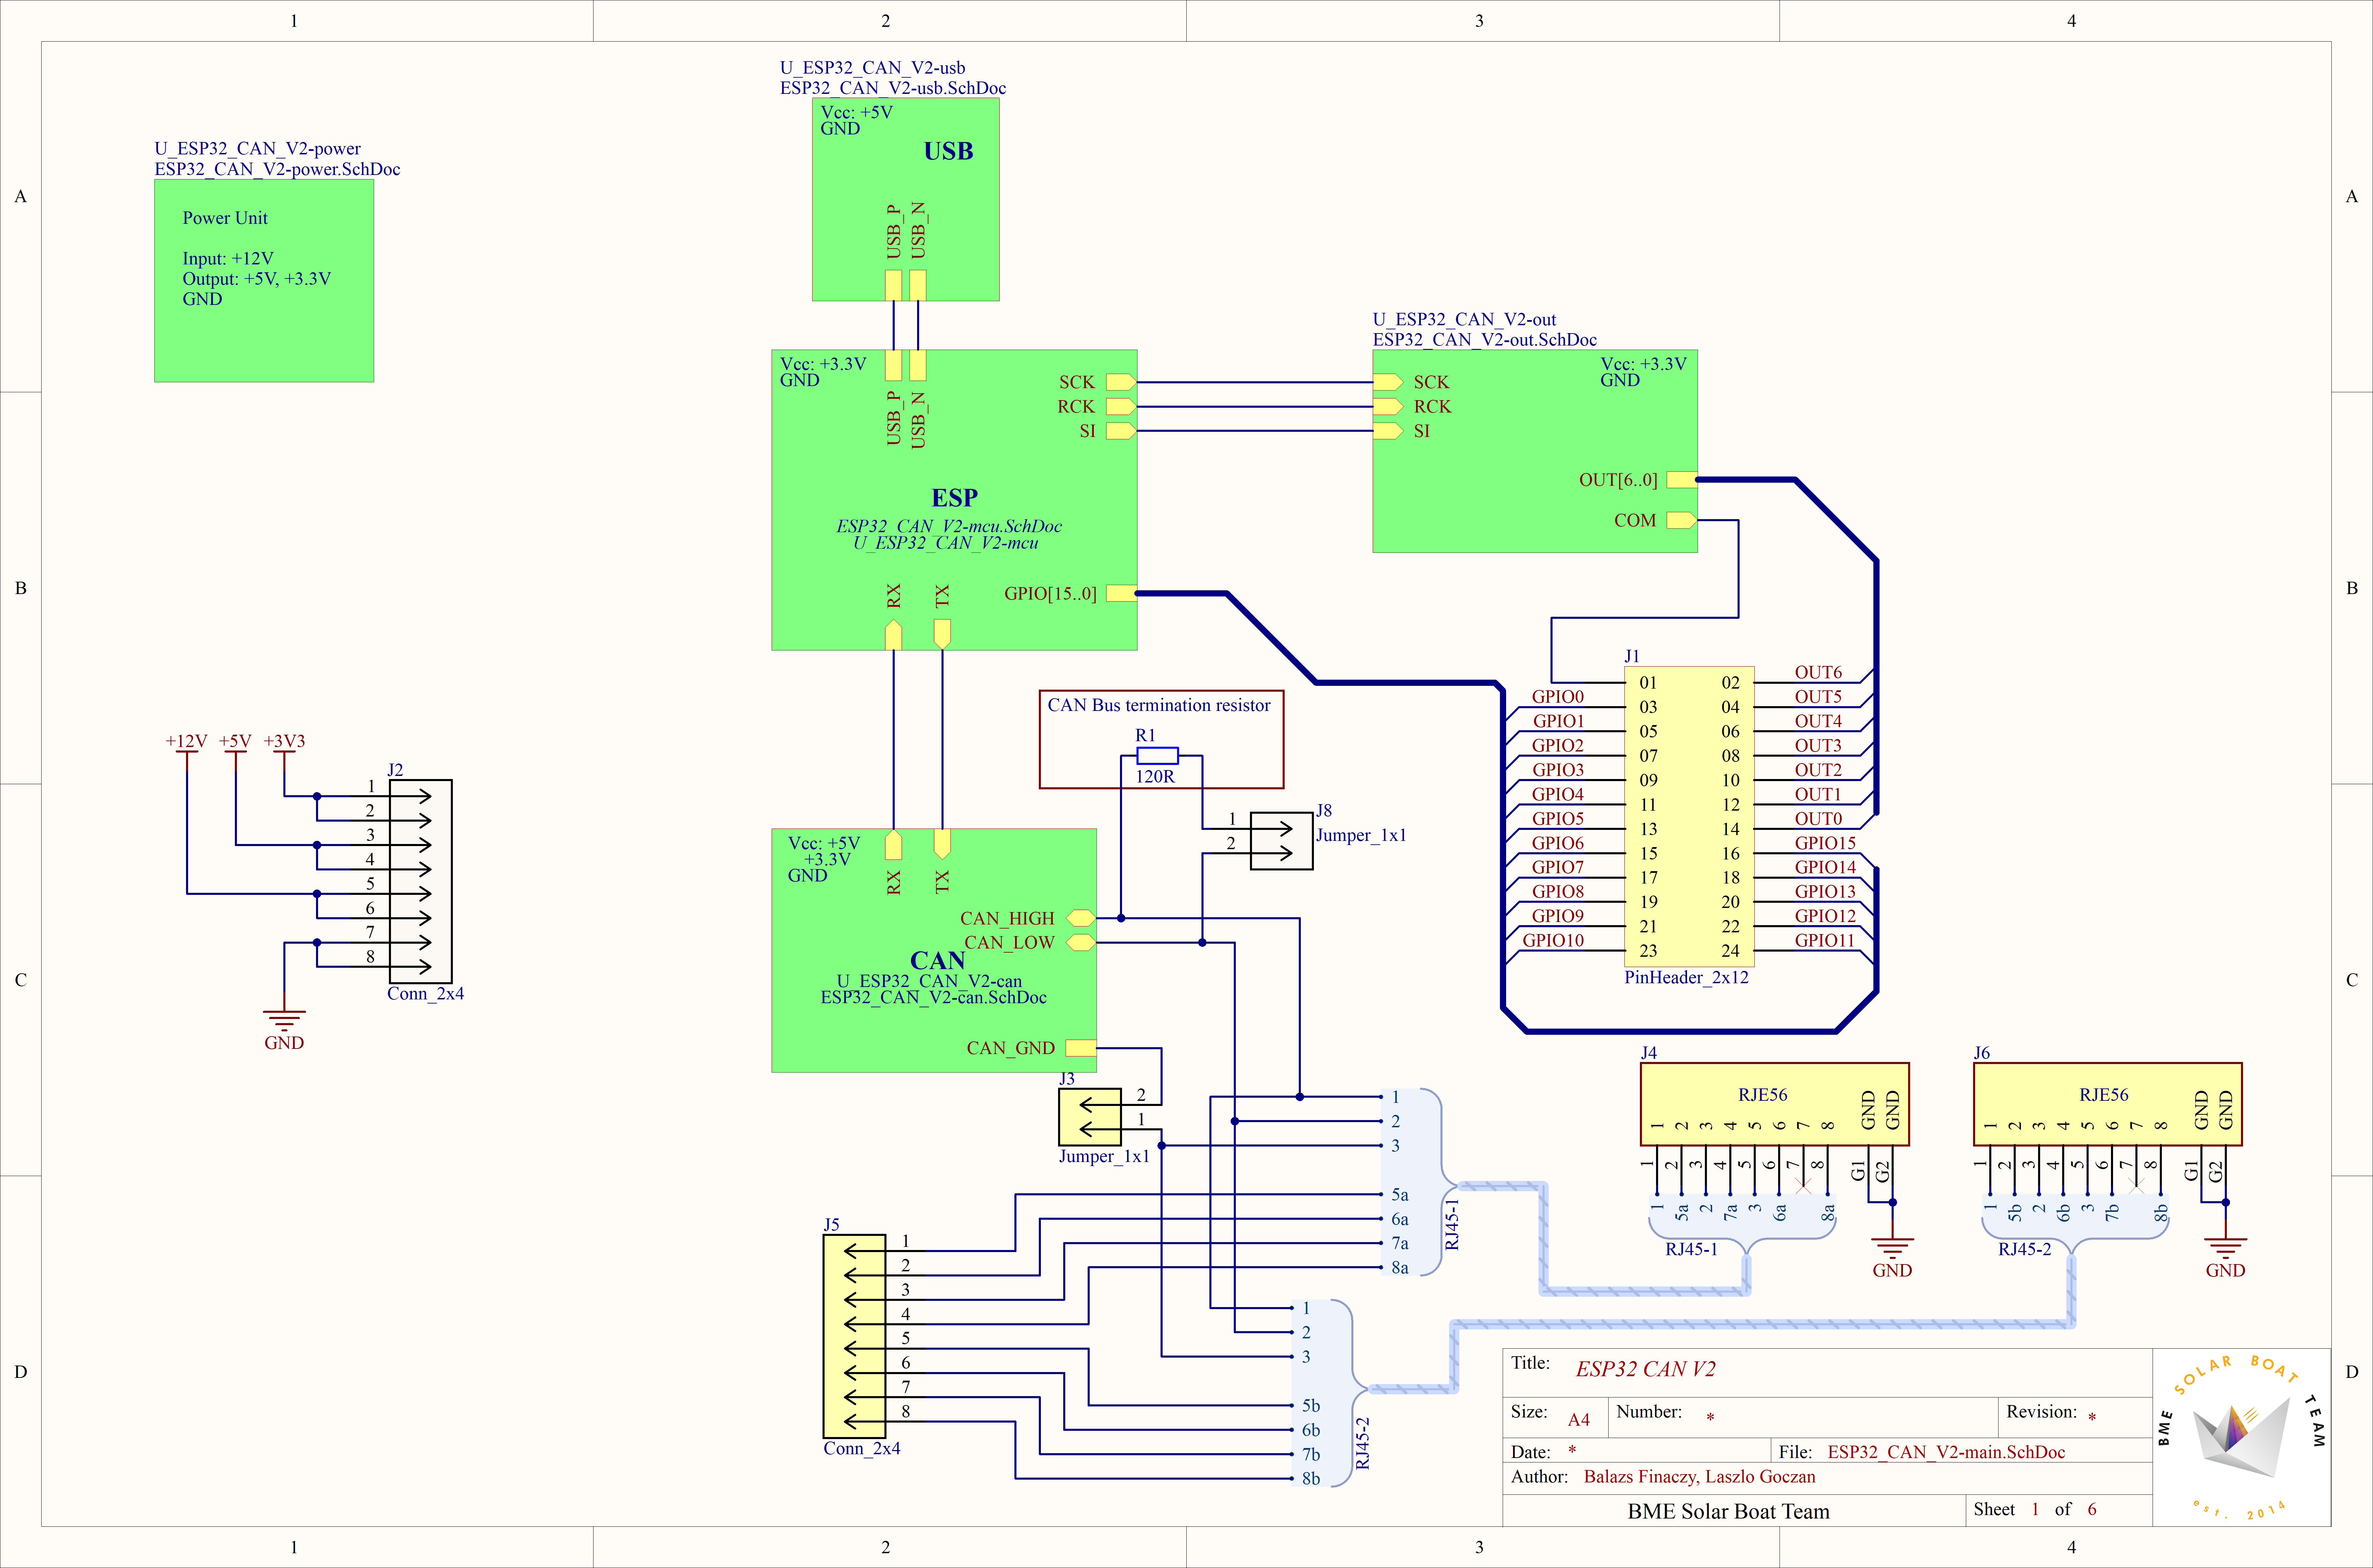
\includegraphics[width=\textwidth]{images/Page0.png}
	\caption{Rendszerdiagram}
	\label{fig:sch_page_0}
\end{figure}

Az egyszerűbb átláthatóság érdekében a a fentebbi ábrán modulonként vannak feltüntetve a különböző alegységek a kapcsolásban. Ezen felül megtalálhatóak a kivezetések még ezen a rajzon.

Az \texttt{R1}-es ellenállás maga a CAN-busznak a lezáróellenállása, amit egy jumperrel rá lehet kötni a buszra vagy sem. Az eredeti kirchoffi rendszer-elméletnek megfelelően nem lenne szükség a megszakító jumperre, azonban a távvezeték hatást figyelembe véve már szükség van rá, hogy ne rontsa el a túl sok, rákötött ellenállás a hullámimpedanciának megfelelően beállított lezárást.

\pagebreak
\subsection{MCU modul}
\begin{figure}[H]
	\centering
	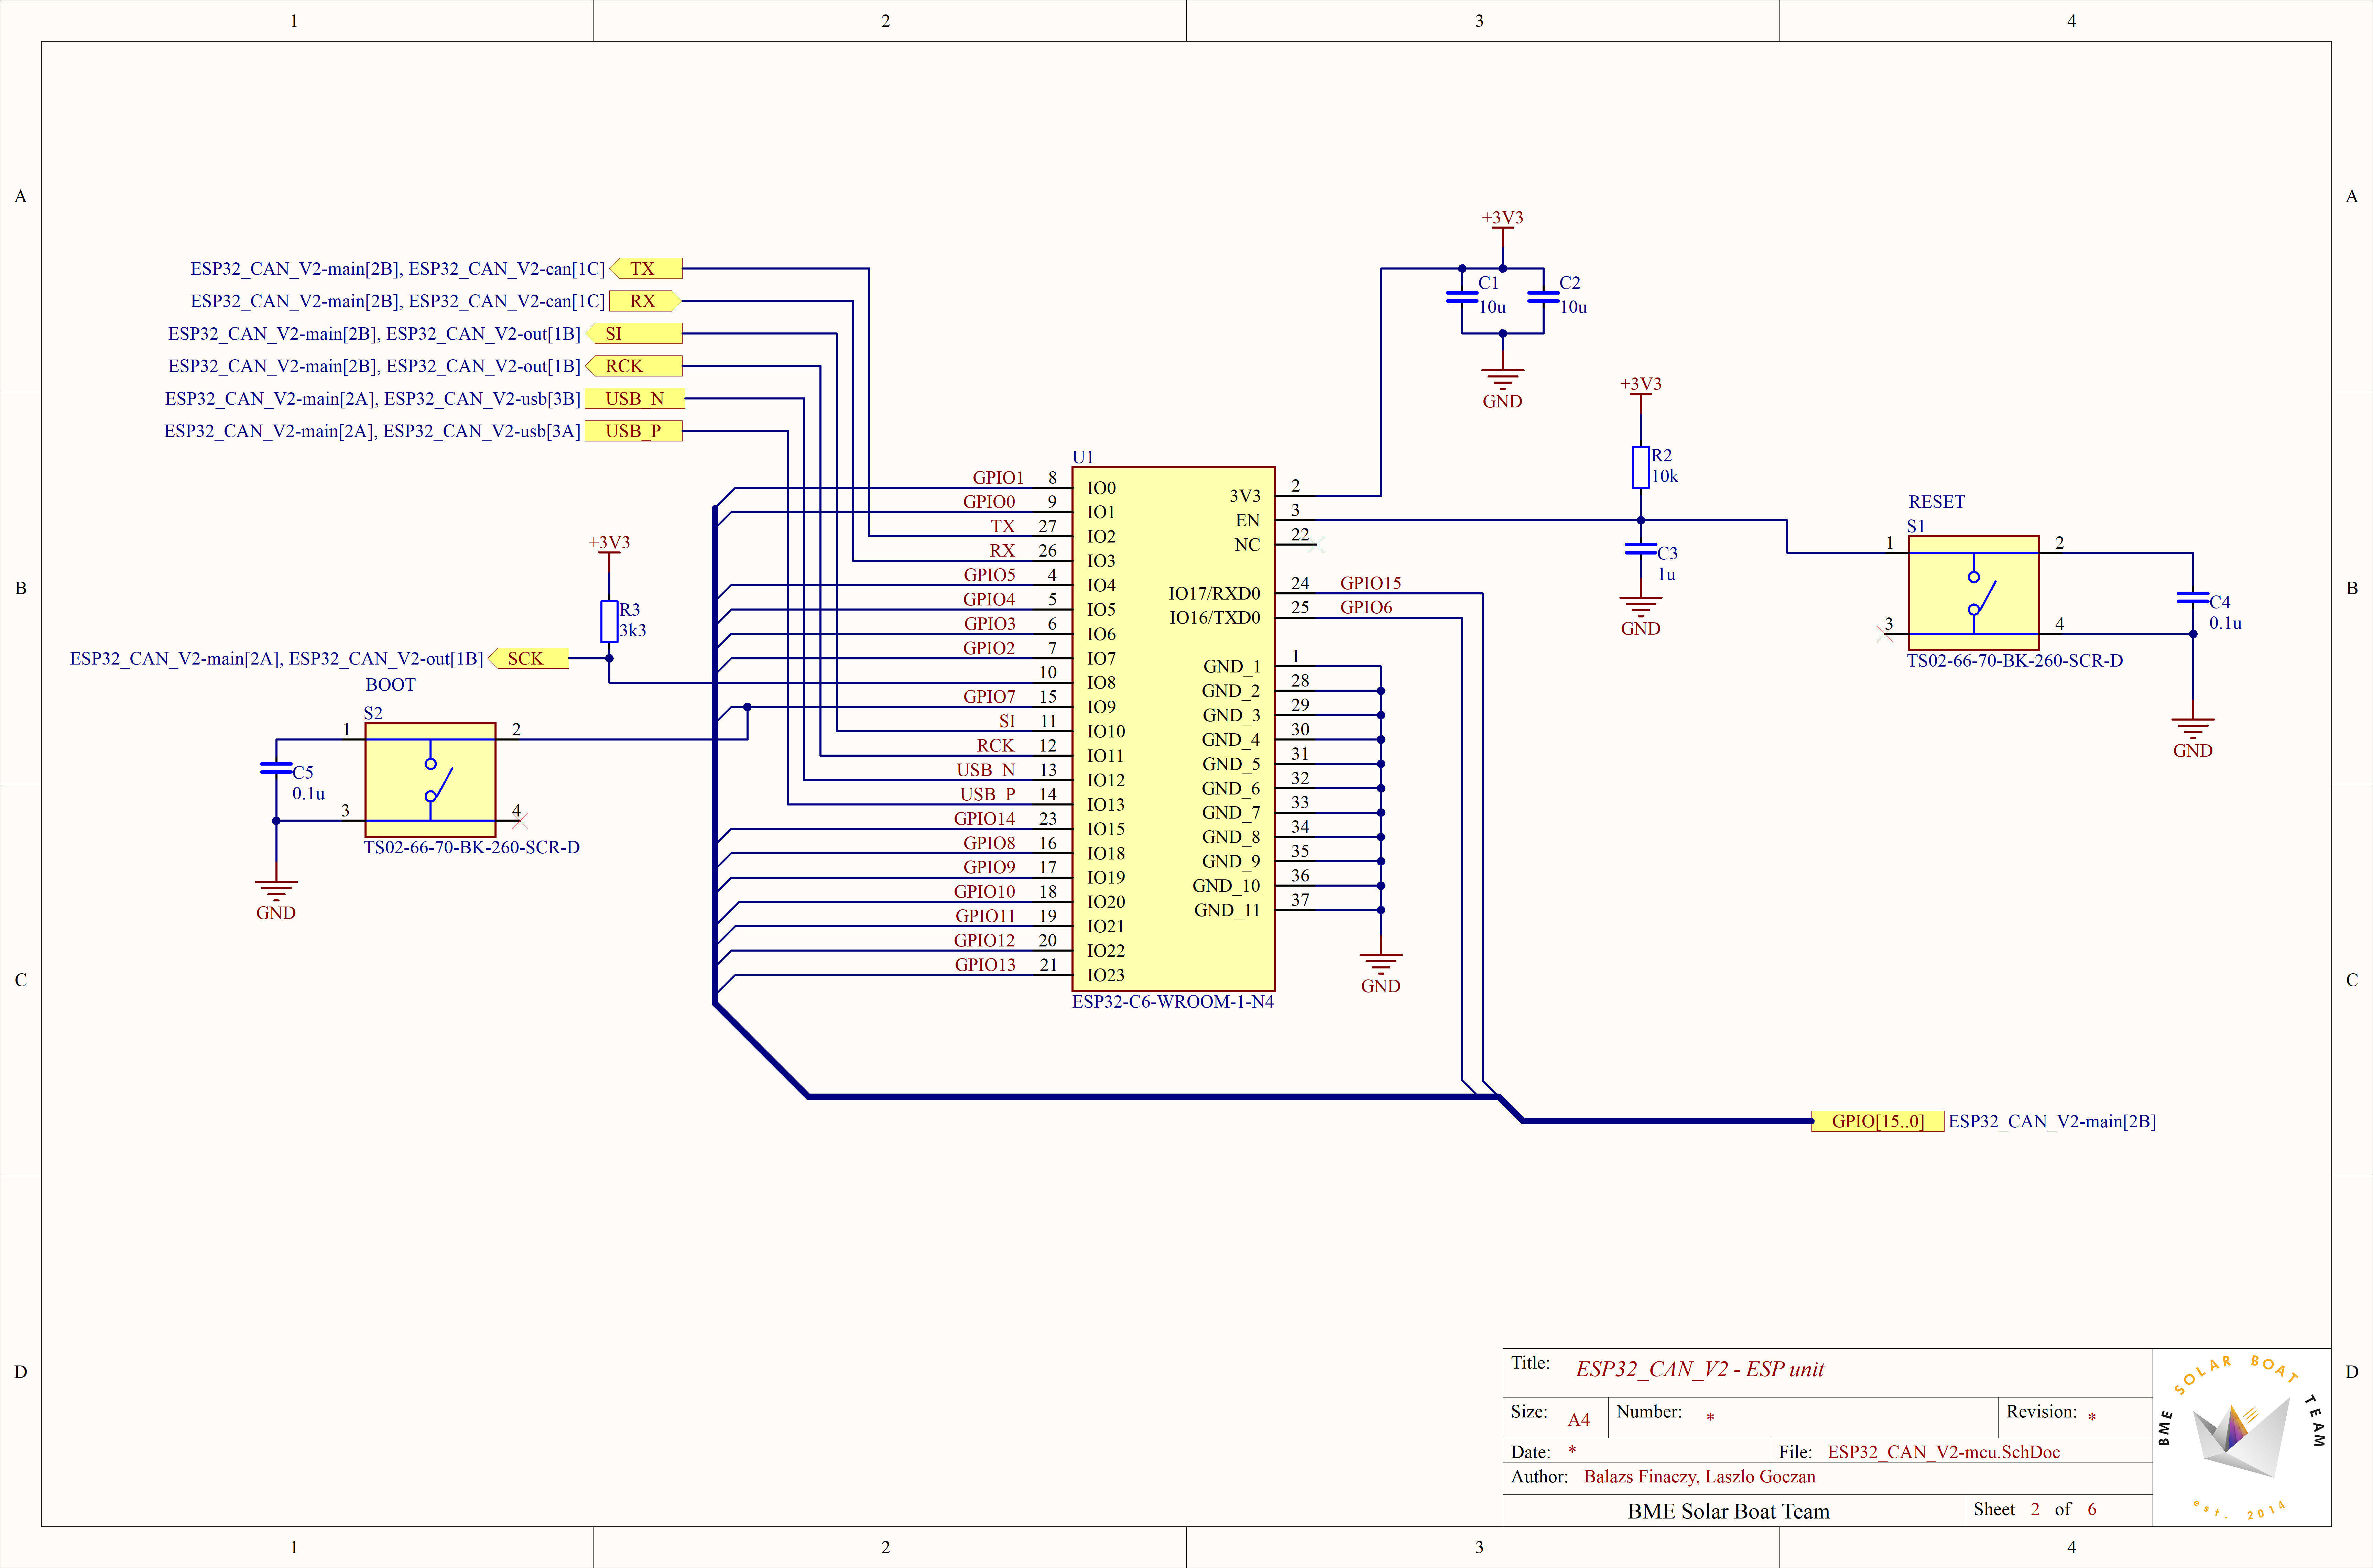
\includegraphics[width=\textwidth]{images/Page1.png}
	\caption{MCU modul}
	\label{fig:sch_page_1}
\end{figure}

A fentebbi ábrán látható az ESP32-C6 és az ahhoz tartozó perifériák bekötése. Az adatlapnak megfelelően tápszűrés lett alkalmazva a táplábon. Ezen felül szintén az adatlap által definiált lábakra bekötésre került egy-egy \texttt{BOOT} és \texttt{RESET} gomb. A különböző alrendszerekkel történő kommunikációt a bal felső sarokban lévő portok alapján lehet értelmezni. Az összes többi \texttt{GPIO} láb kivezetésre került egy tüskesorra, amihez más perifériákat lehet csatlakoztatni.

\pagebreak
\subsection{USB modul}
\begin{figure}[H]
	\centering
	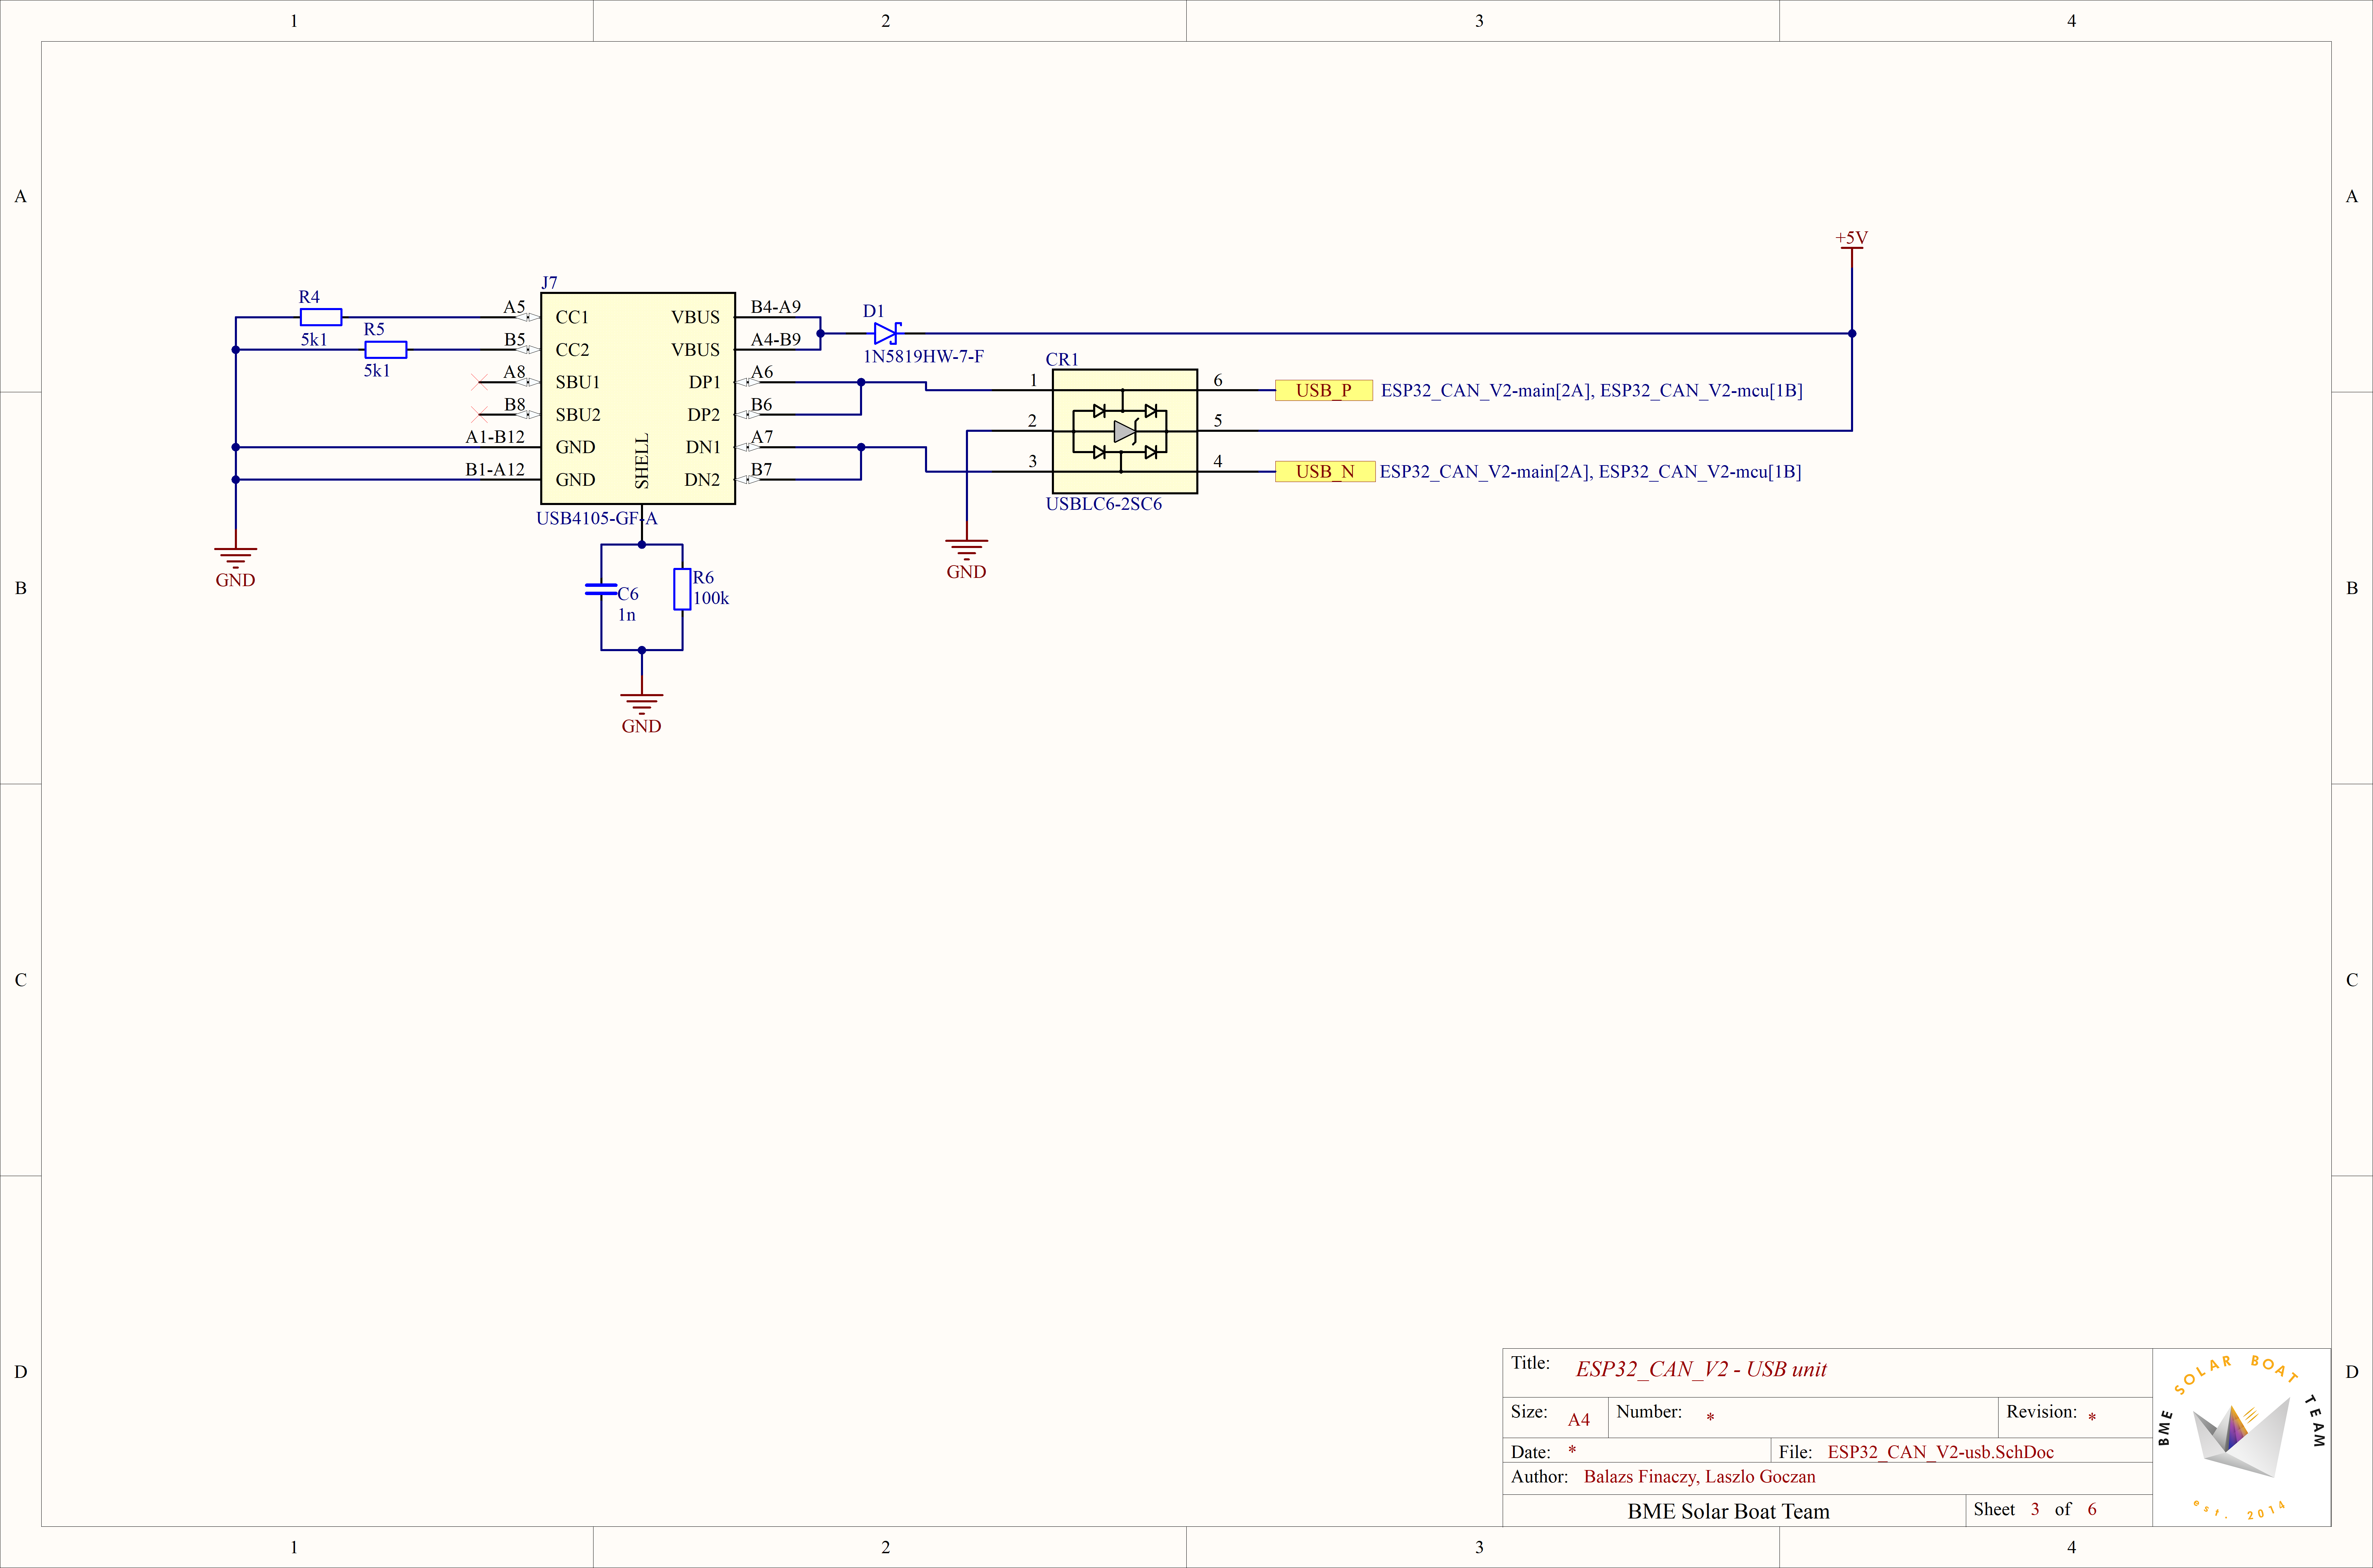
\includegraphics[width=\textwidth]{images/Page2.png}
	\caption{USB modul}
	\label{fig:sch_page_2}
\end{figure}

A mikrokontroller programozásához szükségünk van egy csatlakozóra, amin keresztül a fejlesztőkörnyezet csatlakozni tud az mcu-hoz. Esetünkben a választás egy USB-C csatlakozóra esett. Bár igen aprólékos, és pepecselős munka az ilyen csatlakozók beforrasztása, mégis az eltrejedtsége miatt megérte ezt választani, hogy ne legyünk egy igyen ritka kábelnek kiszolgáltatva.

Látható, hogy a csatlakozó maga csatlakozik az 5V-os táphoz, ami azért van, hogy a különböző védőelektronikáknak ezáltal be tudjuk állítani, hogy az 5V-nál nagyobb feszültségtüskét, feszültségszintet levágja. Ebben játszik szerepet mind a D1-es  Schottky-dióda, ami abban az esetben, ha az anód-oldalán a feszültségszint túlhaladja az 5V + a saját nyitófeszültségének szintjét, úgy azon a szinten levág.

Védelmet nyújt a CR1-es védődióda-csoport is, ami a csatlakozót a mikrokontrollerrel összekötő adatvonalakat védi diódákkal, szintén kiszűrve a negatív és a pozitív feszültségtüskéket.

\pagebreak
\subsection{Kimenetillesztő modul}
\begin{figure}[H]
	\centering
	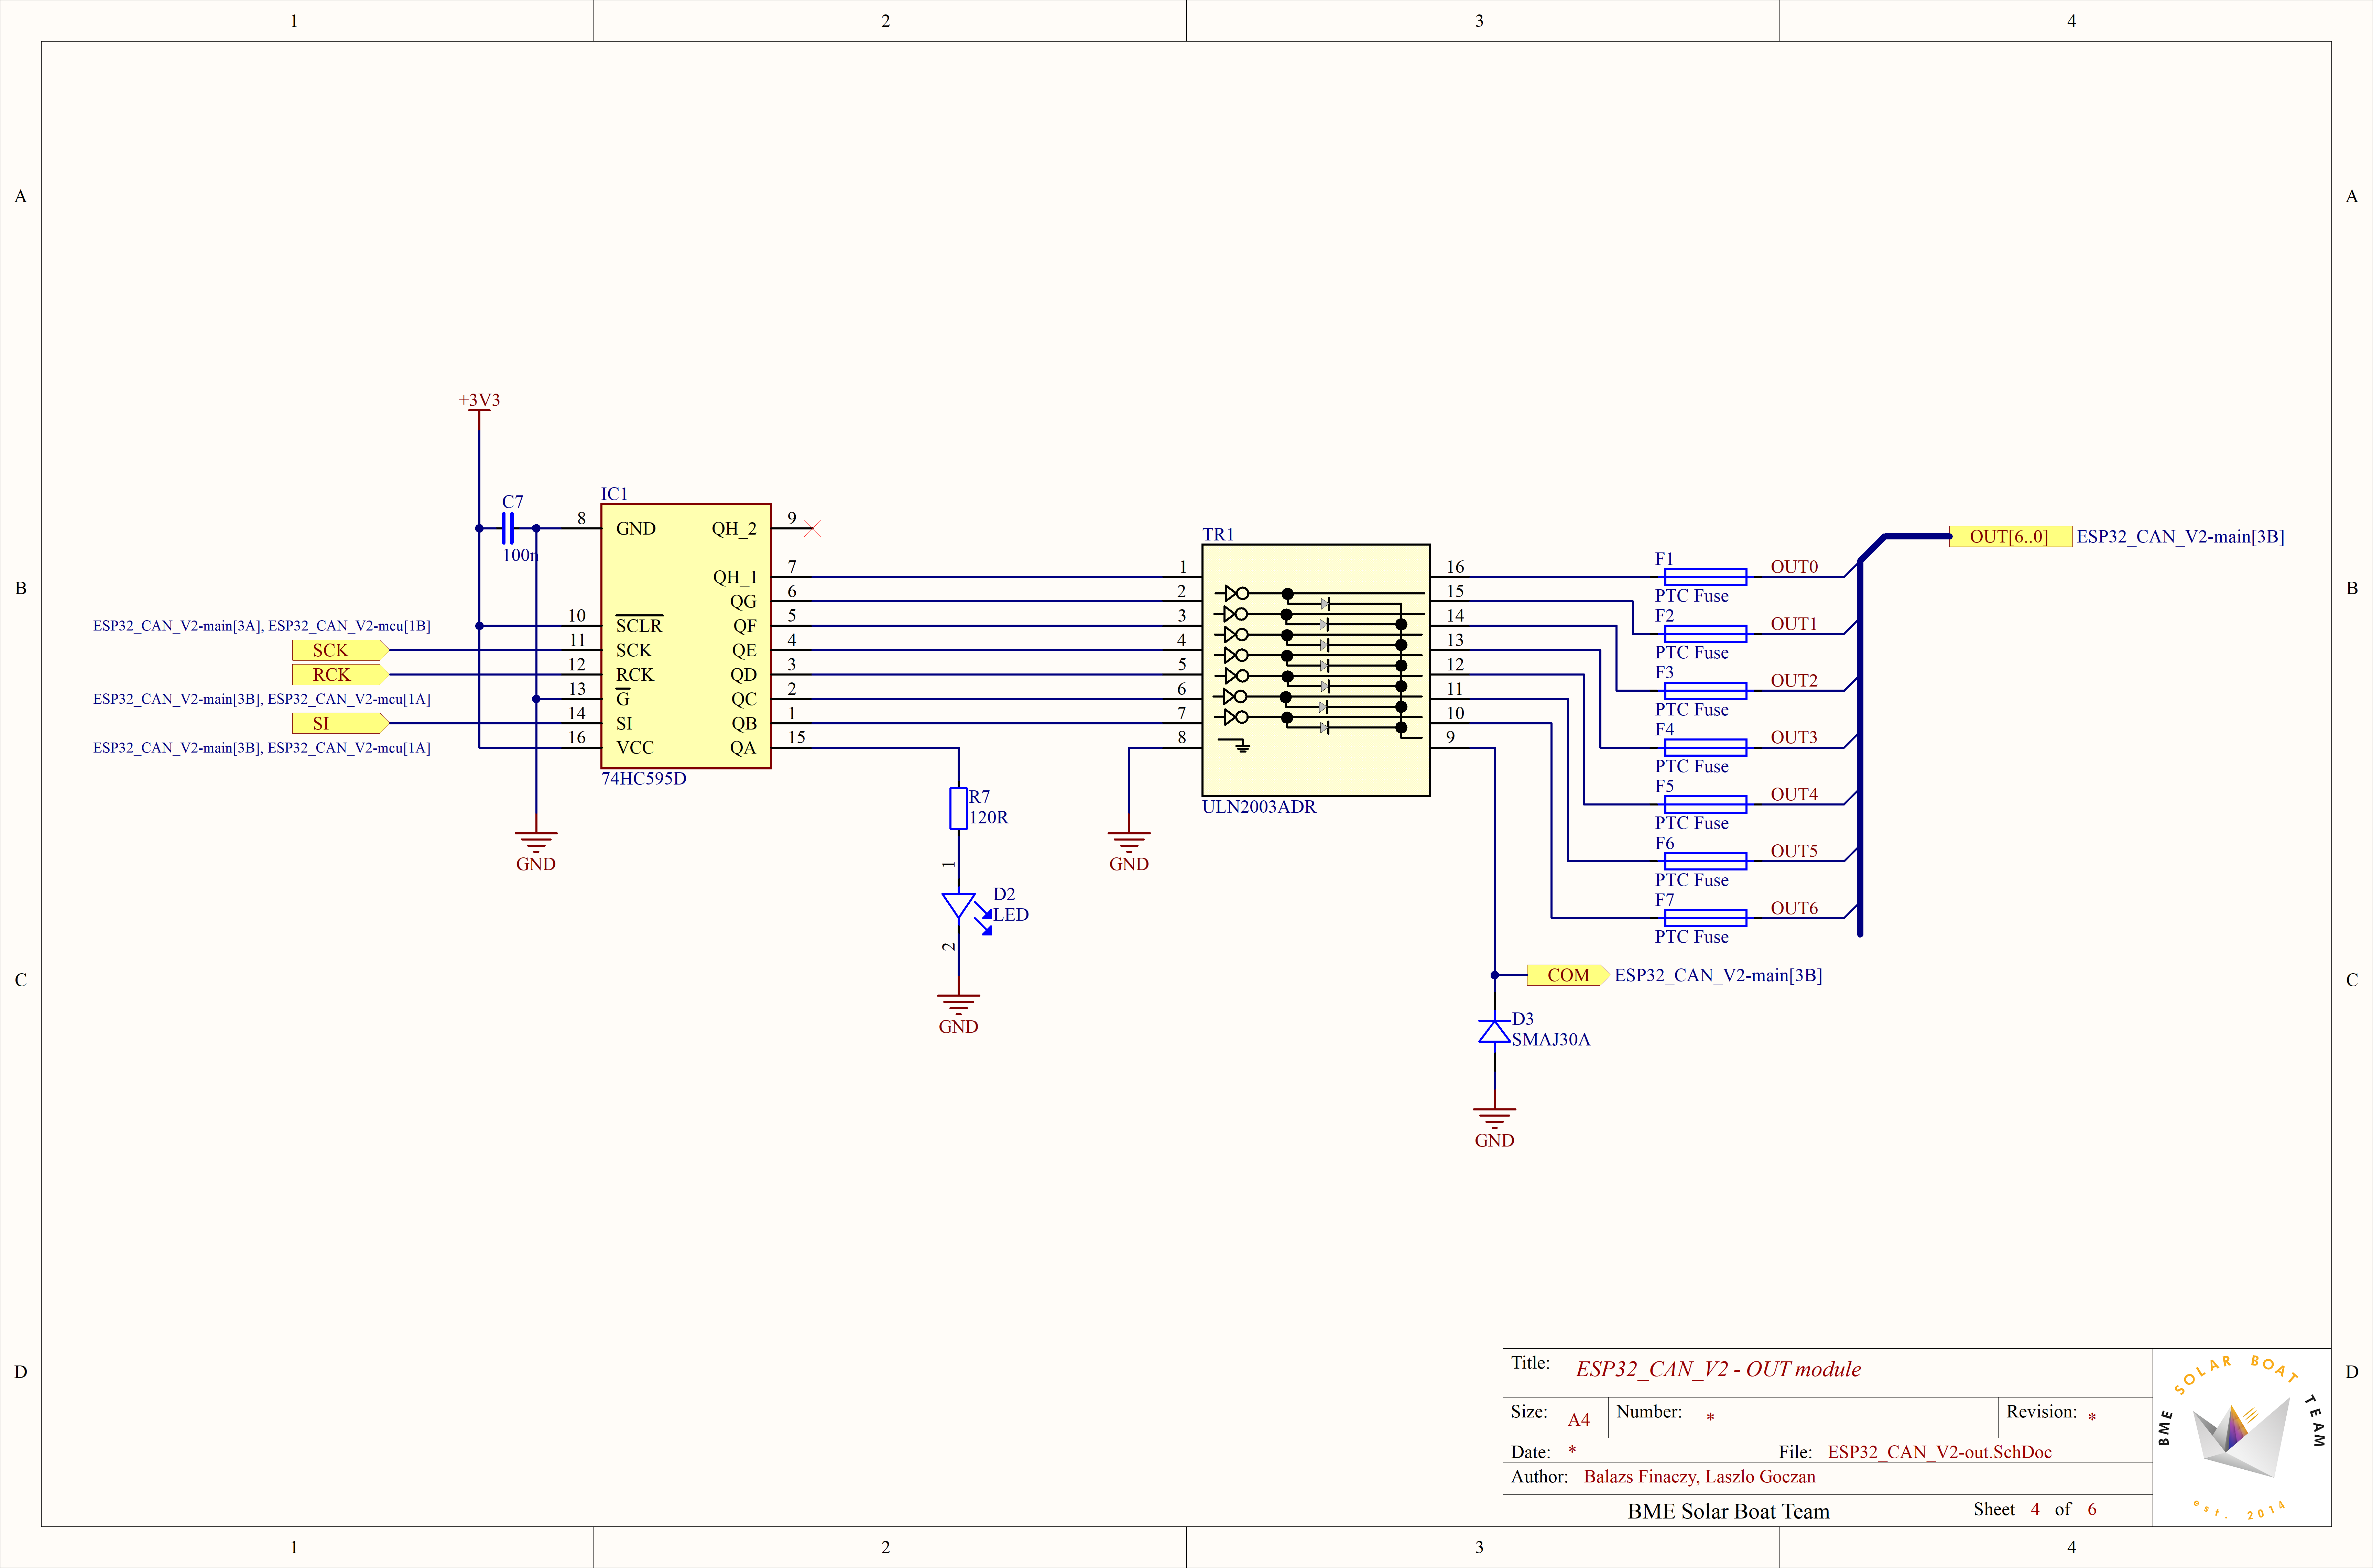
\includegraphics[width=\textwidth]{images/Page3.png}
	\caption{Kimenetillesztő modul}
	\label{fig:sch_page_3}
\end{figure}

Ebben a modulban egy egyszerű shiftregiszterrel bővítjük a mikrokontroller kimeneteit, viszont a kimenetek áramtűrését még ráadásul egy Darlington-kapcsolást tartalmazó IC-vel felbővítjük. Átlagosan egy MCU különböző lábai nagyon maximum 100mA terhelést bírnak el, de ezt a kapcsolást alkalmazva azt felbővítjük egészen 	500mA-ig. Ennek a bővítésnek jelenleg fixen tervezett célja nincs, a lehetőségét szeretnénk meghagyni a későbbiekben annak, hogy nagyobb áramot igénylő kapcsolásokat tudjunk működtetni a panellal.

Vádelemnek mindegyik kimenetre betervezésre került egy SMD E-Fuse, aminek az a lényege, hogy nem elolvad, így, amennyiben az áramkör újraindításra kerül, úgy visszaállnak alapállapotba és nem kell alkatrészt cserélni, viszont megvédte az áramkörünket a túlzott áramfelvétellel szemben.

Magát a Darlington-kapcsolást különböző feszültségszinteken lehet használni. Ezt a célt szolgálja a \texttt{COM}-port, amire akkora feszültségszintet kell kötni, mint amekkorát kapcsolni szeretnénk magával az IC-vel.

\pagebreak
\subsection{Tápkör}
\begin{figure}[H]
	\centering
	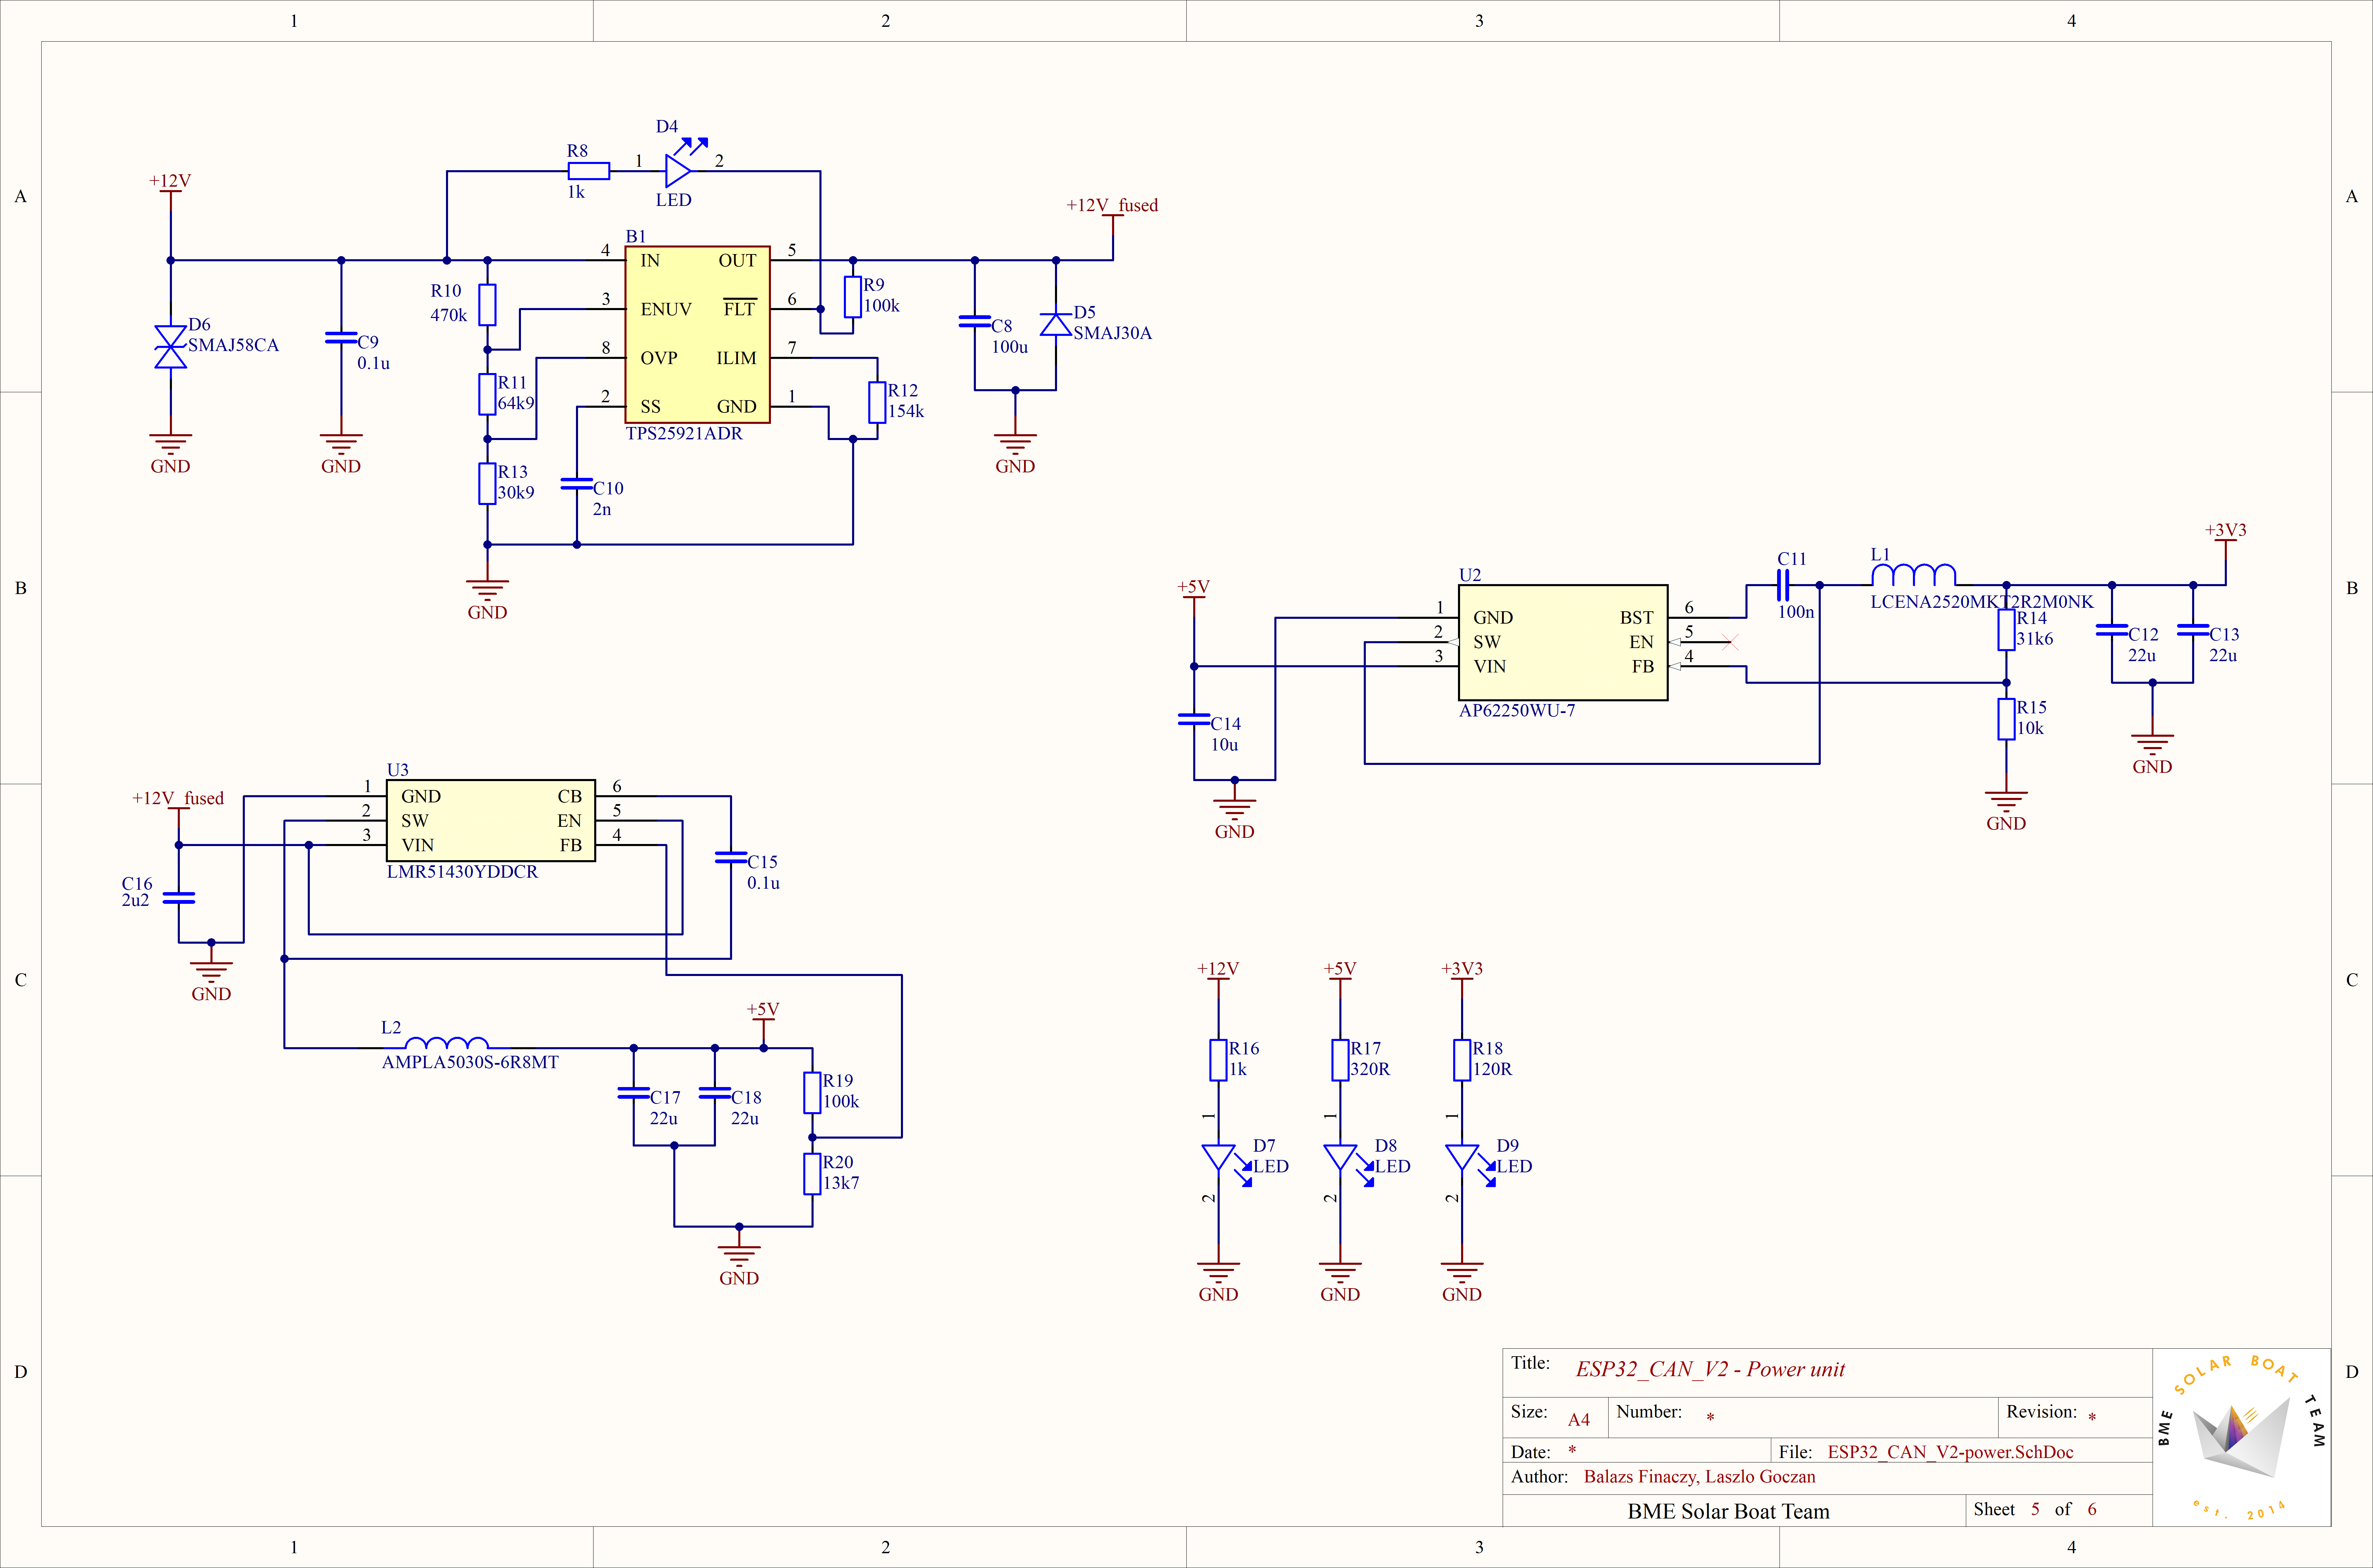
\includegraphics[width=\textwidth]{images/Page4.png}
	\caption{Tápkör}
	\label{fig:sch_page_4}
\end{figure}

A tápkör több fokozatban állítja elő a szükséges feszültségszinteket. Az akkumulátorról 12V-ot kap maga a panel, amit először egy smd polyfuse-on keresztül biztosít túláram és túlfeszültség ellen. Az adatlap alapján számolt értékek, amiket jelenleg alkalmazunk a kapcsolásban 26V-nál, illetve valamennyivel 1A alatti áramfelvétel esetén kapcsol le. Ugyanakkor figyelni kell, mert hozzávetőleg 35V-nál viszont már károsulhat az IC. Ehhez a biztosítékhoz van kötve egy LED is, ami akkor van felkapcsolva, ha a biztosíték lecsapott.

A védelmi fokozaton átvezetett tápot két fokozatban, Buck-converterek konvertálják 5V0-ra, majd pedig 3V3-ra. Az 5V0 feszültségszintre első sorban a CAN-kommunikáció miatt van szükség, a 3V3 pedig az mikrokontroller miatt kell. 

\pagebreak
\subsection{CAN modul}
\begin{figure}[H]
	\centering
	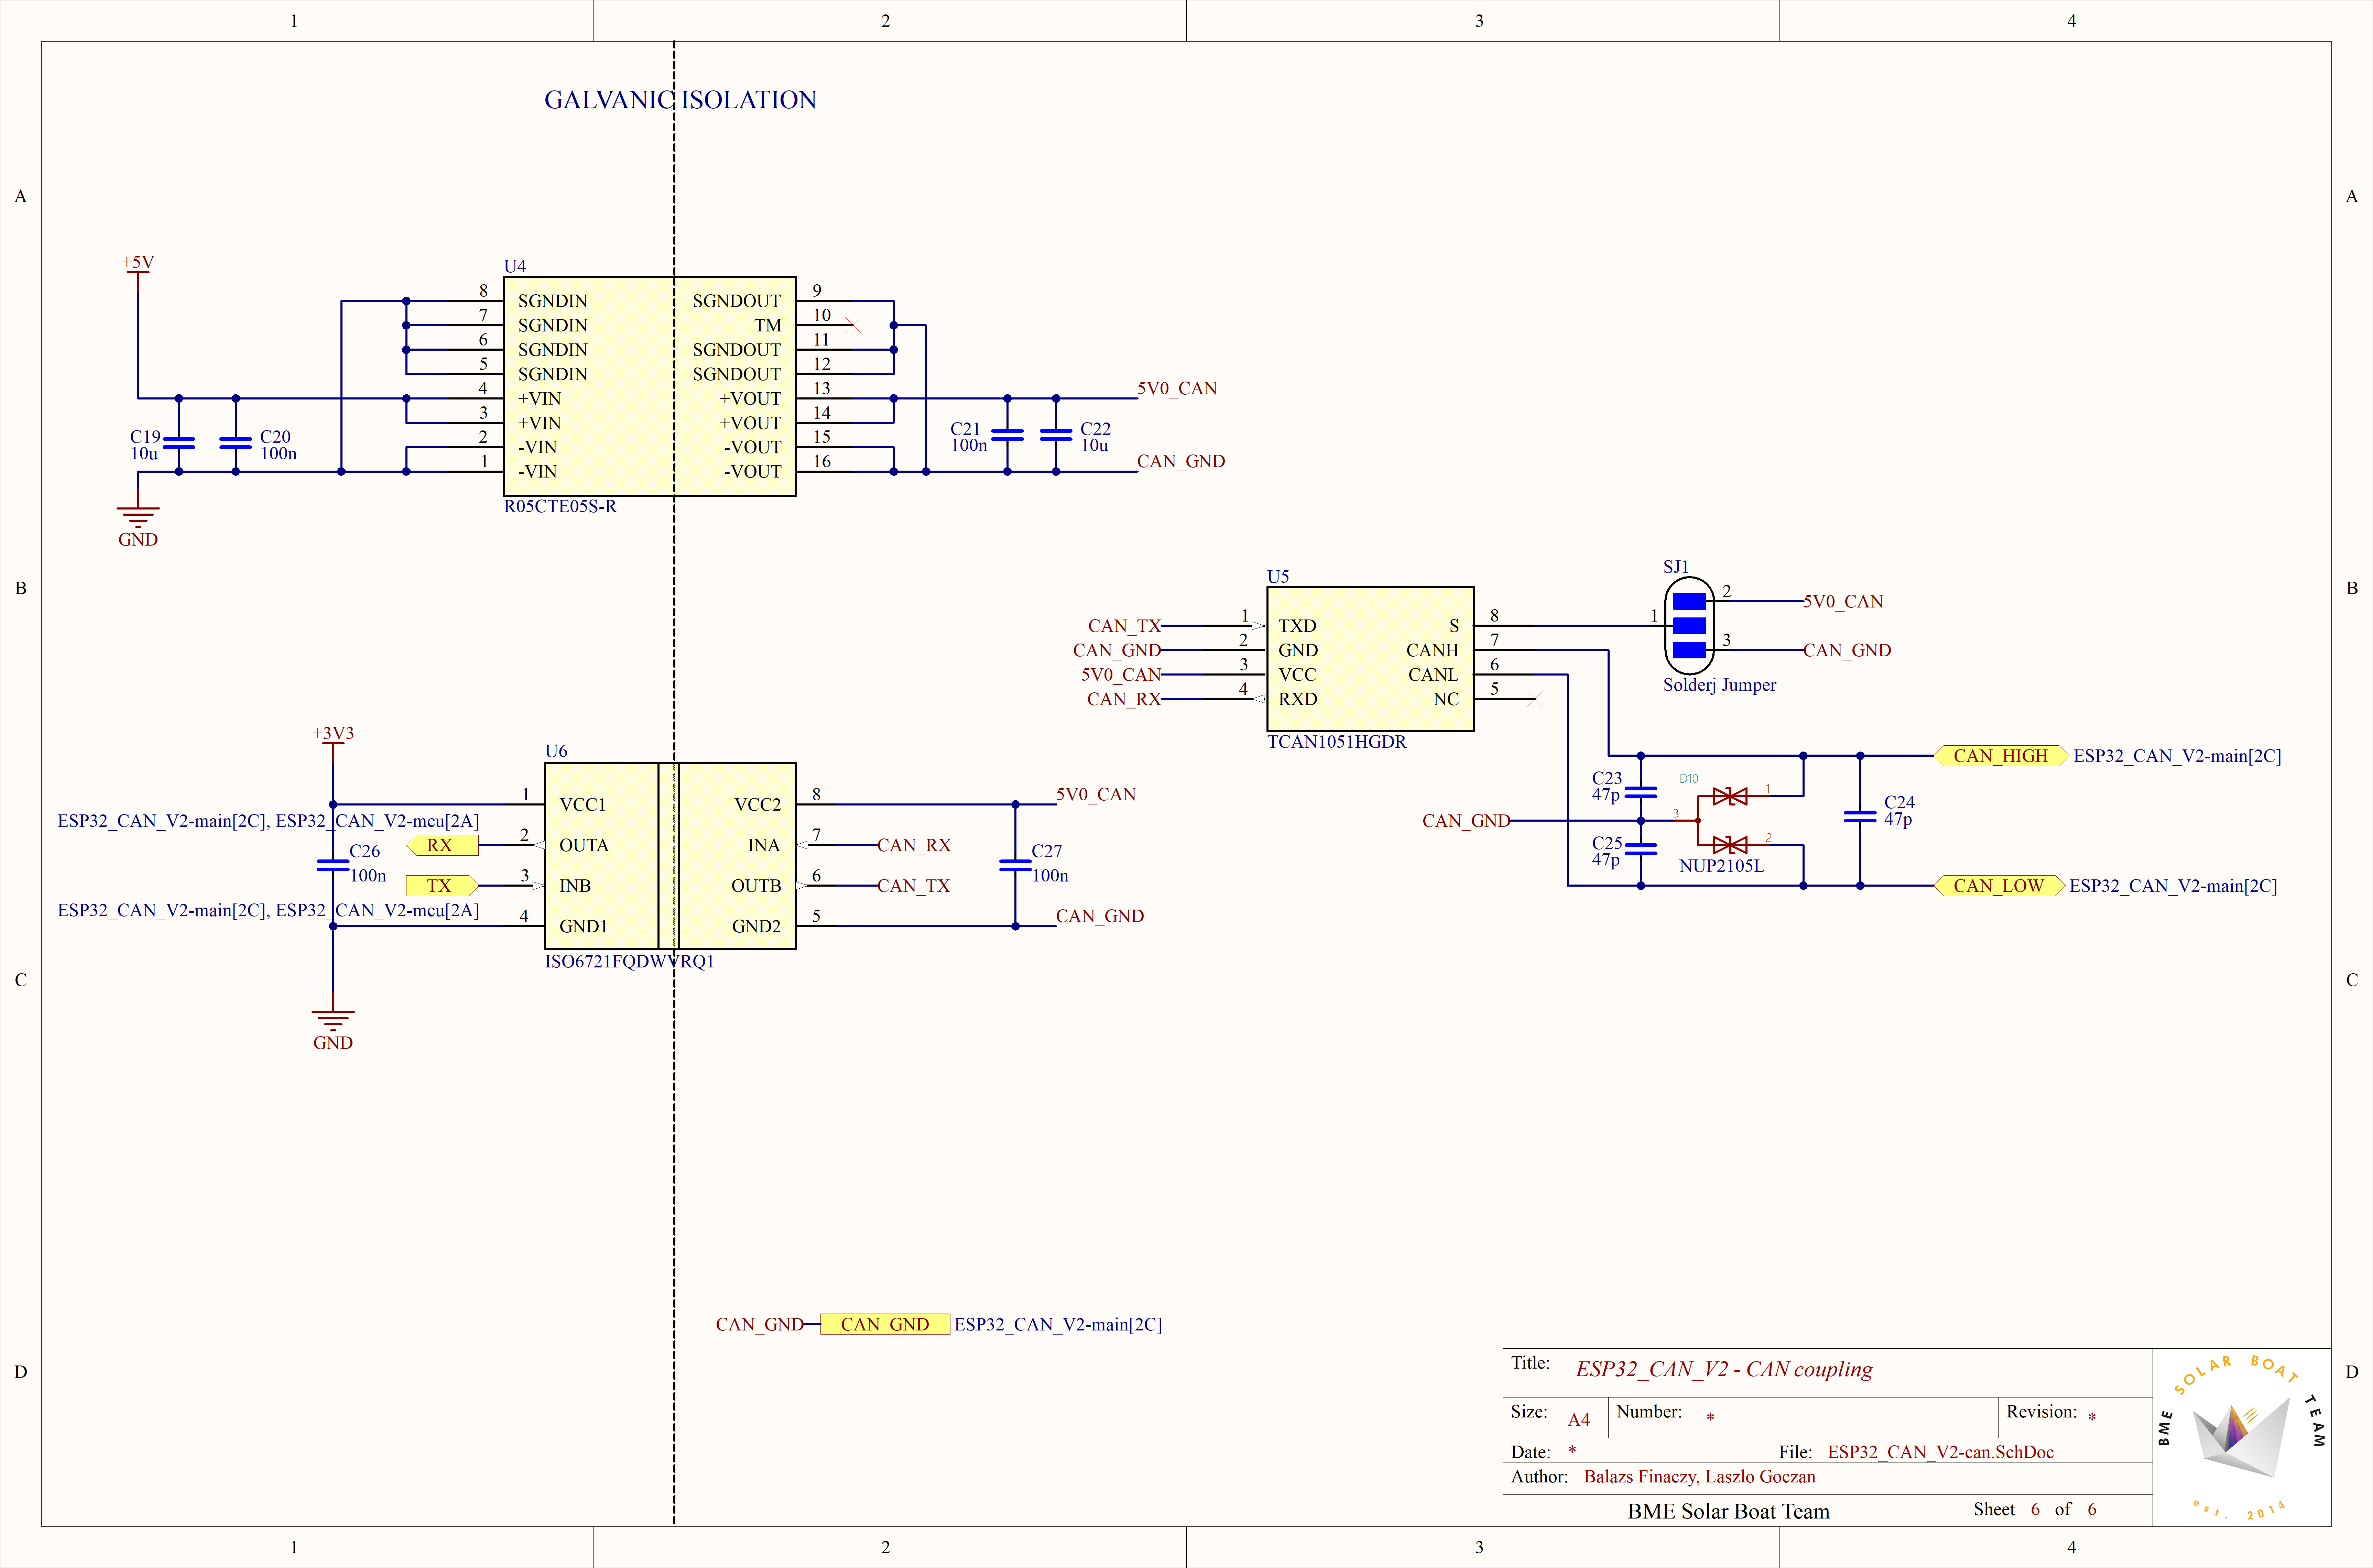
\includegraphics[width=\textwidth]{images/Page5.png}
	\caption{CAN modul}
	\label{fig:sch_page_5}
\end{figure}

A CAN modul első alegysége egy DCDC csatoló, ami galvanikusan leválasztja a CAN-buszt a pcb többi részétől, ez által megelőzve a busz által okozott potenciálkülönbség-problémákat.  Az U6-os IC szintén egy leválasztó egység, ami viszont a mikrokontrollert választja le a buszról. A leválasztott jeleket kapja meg az U5-ös IC, ami maga a CAN-interface. Ő az, aki az MCU-tól kapott UART-üzeneteket kirakja a CAN-buszra, a megfelelő formátumban, illetve a CAN-buszon olvasott üzeneteket UART-protokollnak megfelelően átalakítja és továbbítja az MCU-nak. Ugyanitt van lehetőség az SJ1-es solderjumper megfelelő shortolásával a CAN-busz logikáját is beállítani. Értelem szerűen fontos, hogy egységesen legyen mindegyik node beállítva.